\input{../header.tex}

\subject{VERSUCH NUMMER 400}
\title{Reflexion, Brechung und Beugung}
\date{
  Durchführung: 18.04.2023
  \hspace{3em}
  Abgabe: 25.04.2023
}

\begin{document}

\maketitle
\thispagestyle{empty}
\tableofcontents
\newpage
\setcounter{page}{1}
\section{Ziel}
\label{sec:Ziel}
\section{Theorie}
\label{sec:Theorie}


Die Ausbreitung elektromagnetischer Wellen, also u.a. Licht, lässt sich mit Hilfe der Maxwellgleichungen beschreiben.
Die Reflexion und Brechung an Grenzflächen können durch einfache Gesetze der Strahlenoptik beschrieben werden.
In der Strahlenoptik wird die Wellenausbreitung durch die Wellennormale beschrieben, welche senkrecht auf der Wellenfront und somit parallel zur 
Ausbreitungsrichtung. Die Wellennormale wird als Lichtstrahl bezeichnet.
An Grenzflächen kann die Welle transmittiert oder reflektiert werden.
\subsection{Theoretische Grundlagen zur Reflexion von EM-Wellen.}
\label{sec:Reflexion}
Wenn ein Lichtstrahl auf eine Grenzfläche fällt, so gilt für die Winkelbeziehung 
\begin{equation}
    \alpha_1=\alpha_2\. .
    \label{eqn:Reflex}
\end{equation}
\begin{figure}
    \centering
    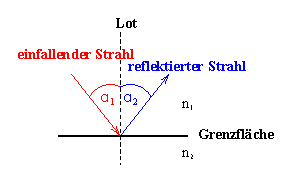
\includegraphics[height=4cm]{Reflexiontheo.pdf}
    \caption{Schematische Darstellung der Reflexion\cite{ap400}.}
    \label{fig:ReflexionTheo}
\end{figure}
\subsection{Theoretische Grundlagen zur Brechung von EM-Wellen.}
\label{sec:Brechung}
Durch verschiedene Ausbreitungsgeschwindigkeiten in verschiedenen Medien, kommt es zur sogenannten Brechung, welche schematisch in \autoref{fig:BrechungTheo} dargestellt ist.
\begin{figure}
    \centering
    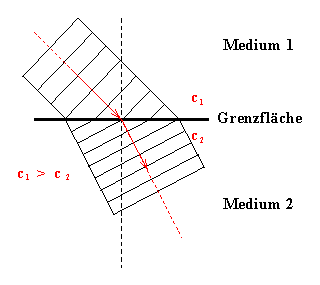
\includegraphics[height = 6cm]{BrechungTheo.pdf}
    \caption{Bildhafte Darstellung einer Brechung einer EM-Welle\cite{ap400}.}
    \label{fig:BrechungTheo}
\end{figure}
Zwischen den beiden Ausbreitungsgeschwindigkeiten $v_1$ und $v_2$ gilt die Beziehung
\begin{equation*}
    \frac{\sin{\alpha}}{\sin{\beta}}= \frac{v_1}{v_2}=\frac{n_2}{n_1}\. .
\end{equation*}
Hier bei ist $\alpha$ der Einfallswinkel, $\beta$ der Brechungswinkel und $n$ der jeweilige Brechungsindex des Materials.
In Luft hat Licht die Ausbreitungsgeschwindigkeit $v_1= 2.9979\cdot 10^8 \frac{\unit{m}}{\unit{s}}$, wobei Luft einen Brechungsindex von 
$n_1= 1.000292$
Diese Richtungsänderung der Elektromagnetischen Welle wird durch das Gesetz von Snellius beschrieben
\begin{equation}
    n_1\sin{\alpha}=n_2sin{\beta}\. .
    \label{eqn:snellius}
\end{equation}

\subsection{Theoretische Grundlagen zur Reflexion und Transmission von EM-Wellen.}
\label{sec: Rfelxion und Transmission}
Natürlicherweise treten an Grenzflächen immer Reflexionen und Transmissionen zeitgleich auf, sodass ein Teil des eintreffenden Lichtes reflektiert $R$ und 
der übrige Teil transmittiert $T$ .
Welchen Anteil des eintreffendes Lichts die jeweilige Aktion hat, ist materialabhängig, jedoch gilt stets $R+T=1$.

\begin{figure}
    \centering
    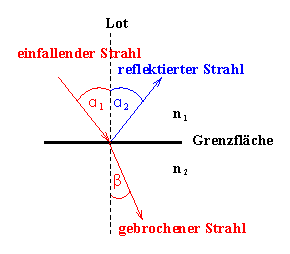
\includegraphics[height= 4cm]{ReflexuTransm.pdf}
    \label{fig:ReflexuTransmTheo}
    \caption{Schematische Darstellung der Reflexion und Transmission\cite{ap400}.}
\end{figure}

\subsection{Theoretische Grundlagen zur Beugung von EM-Wellen.}
\label{sec:BeugungTheo}
Wenn die eine EM-Welle auf ein Objekt trifft, kann häufig beobachtet werden, dass sich diese im Schattenraum ausbreitet.
Also ist die Welle oder in diesem akuten Fall das Licht an Stellen detektierbar, welche es nach der Strahlenoptik nicht erreichen dürft.
Um dieses Phänomen beschreiben zu können, muss die Wellenoptik betrachtet werden.
Eine EM-Welle wird durch ihre Wellenlänge $\lambda$ und ihre Frequenz $\nu$ beschrieben. Wenn es zur Überlagerung mehrerer Wellen kommt, addieren sich die Amplituden
gemäß des Superpositionsprinzip.
Wenn die unterschiedlichen Wellen nun eine Frequenz gemein haben, kann ein Interferenzbild entstehen. Hierbei wird grundsätzlich zwischen destruktiver und konstruktiver Interferenz unterschieden.
Nach dem Huygenschen Prinzip gilt, dass jeder Punkt einer Welle Ausgang einer neuen Elementarwelle ist und die überlagerung dieser eine neue Wellenfront erzeugen.
Trifft eine Welle auf einen Spalt mit Breite $a$, werden alle Punkte in der Spaltöffnung gebeugt und erzeugen so auf einem  Schirm mit Abstand $L$ ein Interferenzmuster.
Die Streifen die konstruktive Interferenz erfahren, erscheinen dann an den Stellen
\begin{equation*}
    a\, \sin{\alpha}=k \lambda  \text{ mit Wellenlänge }\lambda\. .
\end{equation*}
Die Variable $k$ steht hierbei für die Ordnung des Maximums.
Für ein Strichgitter gilt so analog
\begin{equation*}
    d\, \sin{\alpha}=k \lambda \. .
\end{equation*}
Die Größe $d$ wird Gitterkonstante genannt.
\section{Aufbau}
\label{sec:Aufbau}

Die Messapparatur besteht aus einer transparenten Grundplatte und zwei Laserdiodenmodulen.
Diese lassen sich auf einem Halbkreis bewegen, sodass sich der Einfallswinkel einstellen
lässt. Der Aufbau des Versuchs ist in \autoref{fig:aufbau} abgebildet. 

\begin{figure}
    \centering
    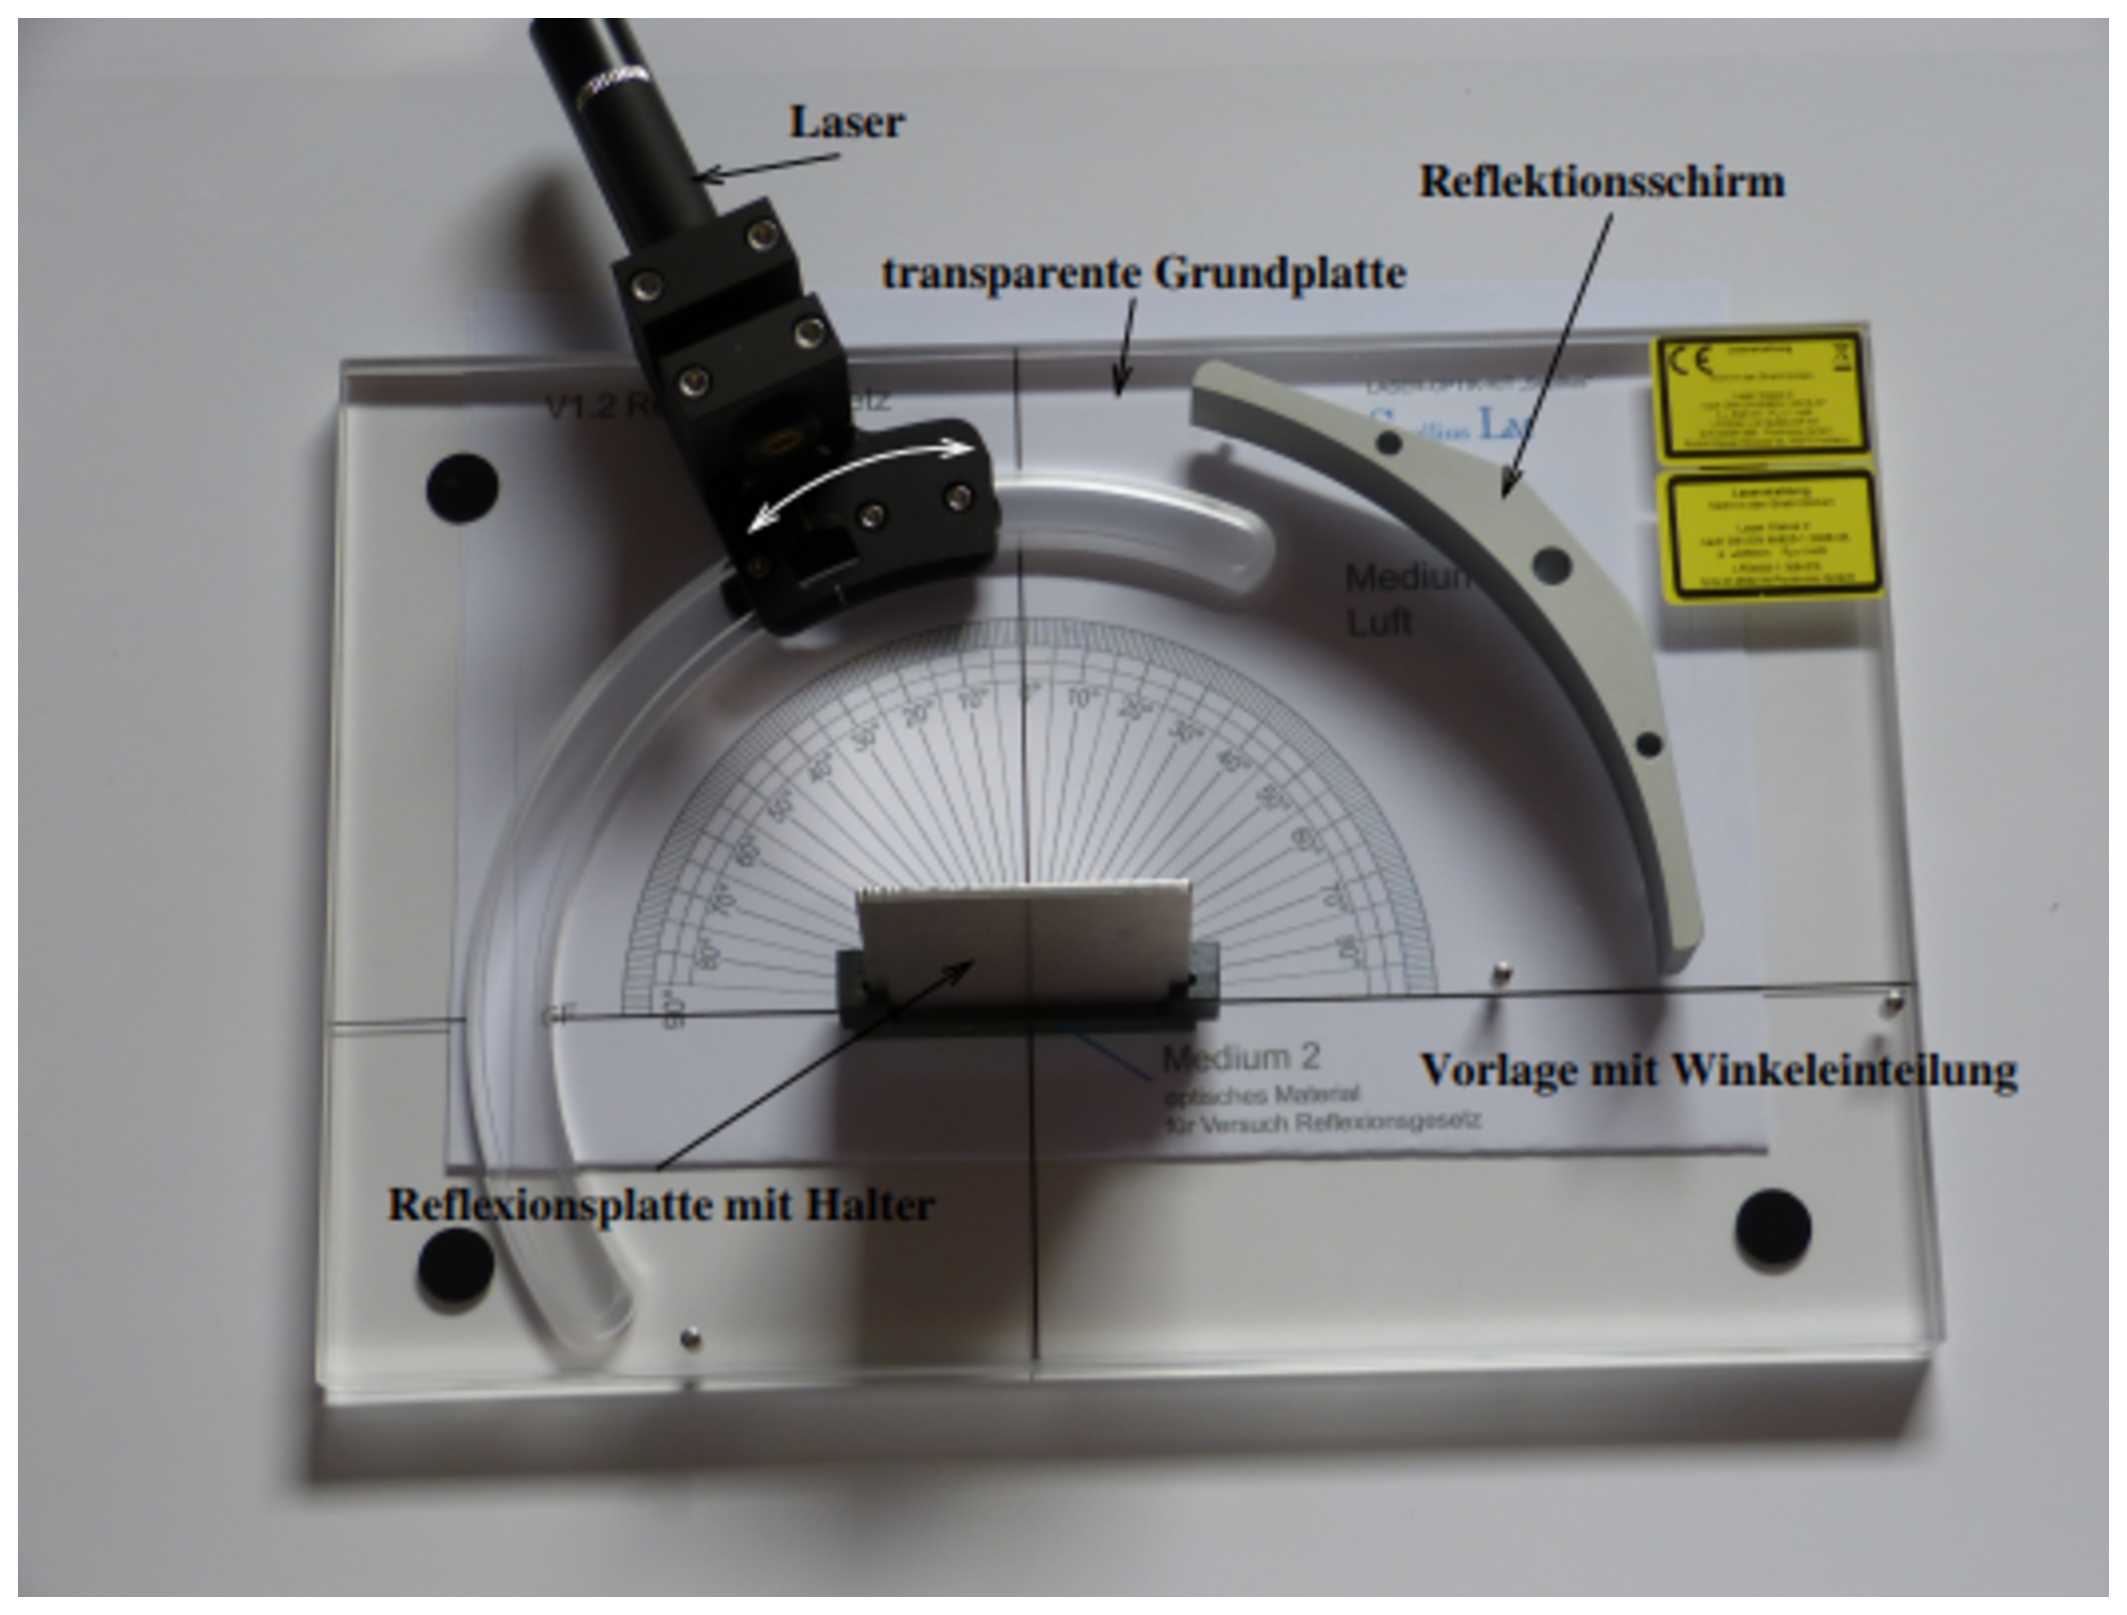
\includegraphics[height = 6cm]{Aufbau.pdf}
    \caption{Aufbau zur Messung von Reflexion, Brechung und Beugung \cite{ap400}.}
    \label{fig:aufbau}
\end{figure}

In der Mitte des Halbkreises lassen sich verschiedene geometrische Elemente platzieren,
die in \autoref{fig:figuren} abgebildet sind. 

Desweiteren befindet sich an der Messapparatur ein Reflexion, der erhöht werden kann.
Bei der Untersuchung der Brechung und der Transmission kann ein Transmissionsschirm 
aufgestellt werden. Außerdem können unter die transparente Grundplatte Vorlagen für
die einzelnen Teilversuche gelegt werden.
\section{Durchführung}
\label{sec:Durchführung}

\subsection{Versuchsteil zum Reflexionsgesetz}
Im ersten Versuchsteil wird ausschließlich der grüne Laser verwendet. Es wird die 
Vorlage A unter der Grundplatte platziert. Ein Spiegel wird in der Mitte der Platte befestigt.
Dann werden für sieben verschiedene Einfallswinkel $\alpha_1$ die Reflexionswinkel
$\alpha_2$ gemessen.

\subsection{Versuchsteil zum Brechungsgesetz}
\label{sec:Brechung}
Auch in diesem Versuch wird ausschließlich der grüne Laser und die Vorlage A verwendet.
Der Spiegel wird nun mit einer planparallelen Platte ersetzt, die so positioniert wird,
dass der Eintrittsspalt zur Winkelskala zeigt und der Winkel des gebrochen Strahl an der
gegenüberliegenden, auf der planparallelen Platte aufgeklebten Skala abgelesen werden
kann. Nun werden für sieben verschiedene Einfallswinkel $\alpha$ die Brechungswinkel
$\beta$ bestimmt.

\subsection{Versuch zur Bestimmung des Strahlversatzes}
Der Versuch wird analog zu \autoref{sec:Brechung} aufgebaut. Zusätzlich wird der
Transmissionsschirm mit Winkelskala angebracht. Nun werden für fünf verschiedene
Einfallswinkel $\alpha$ erneut die Brechungswinkel $\beta$ gemessen. Aus diesen wird
dann der Strahlversatz $s$ bestimmt.

\subsection{Messung der Ablenkung durch ein Prisma}
Diesmal wird sowohl der grüne wie der rote Laser verwendet. Zusätzlich wird die Vorlage C und das Prisma benötigt. 
Außerdem muss der Reflexionsschirm erhöht werden. Für fünf Einfallswinkel $\alpha_1$ zwischen 10° und 60° werden die Austrittswinkel $\alpha_2$ bestimmt. Dies wird einmal
mit dem grünen und einmal mit dem roten Laser gemessen. Dabei müssen die gleichen Einfallswinkel verwendet werden. 

\subsection{Beugung am Gitter}
Zuerst muss der Versuch ohne das Beugungsgitter justiert werden. Dazu muss das Laserlicht die Winkelskala des Transmissionsschirms bei 0 Grad treffen. Zudem muss der 
Transmissionsschirm im Kreis um die Winkelskala der Vorlage angeordnet sein. Nun wird das Gitter mit 600 Linien/mm in die Halterung eingesetzt und es werden die 
Beugungsmaxima für den roten und den grünen Laser ausgemessen. Der Versuch wird mit zwei weiteren Gittern wiederholt. Daraus kann nun die Wellenlänge der beiden Laser 
bestimmt werden.
\section{Auswertung}
\label{sec:Auswertung}
Aufgrund der groben Skala des Winkelmessers, kann der jeweilige Messwert nur mit einem absoluten Fehler von $\pm 1\, \unit{\degree}$ gemessen
werden. Diese Abweichung wurde in den jeweiligen Tabellen direkt mitangegeben.
\subsection{Fehlerrechnung}
\label{sec:Fehlerrechnung}
Für die Fehlerrechnung werden folgende Formeln aus der Vorlesung verwendet.
für den Mittelwert gilt
\begin{equation}
    \overline{x}=\frac{1}{N}\sum_{i=1}^N x_i ß\; \;\text{mit der Anzahl N und den Messwerten x} 
    \label{eqn:Mittelwert}
\end{equation}
Der Fehler für den Mittelwert lässt sich gemäß
\begin{equation}
    \increment \overline{x}=\frac{1}{\sqrt{N}}\sqrt{\frac{1}{N-1}\sum_{i=1}^N(x_i-\overline{x})^2}
    \label{eqn:FehlerMittelwert}
\end{equation}
berechnen.
Wenn im weiteren Verlauf der Berechnung mit der fehlerhaften Größe gerechnet wird, kann der Fehler der folgenden Größe
mittels Gaußscher Fehlerfortpflanzung berechnet werden. Die Formel hierfür ist
\begin{equation}
    \increment f= \sqrt{\sum_{i=1}^N\left(\frac{\partial f}{\partial x_i}\right)^2\cdot(\increment x_i)^2}.
    \label{eqn:GaussMittelwert}
\end{equation}

\subsection{Reflexionsgesetz}
\label{sec:Reflexionsgesetz}

\begin{table}
    \centering
    \caption{Messwerte für die Untersuchung des Reflexionsgesetzes.}
    \begin{tabular}{c c}
        \toprule
        Eintrittswinkel $\alpha_1 \mathrm{/} \unit{\degree}$  & Austrittswinkel $\alpha_2 \mathrm{/} \unit{\degree}$\\
        \midrule
        20\pm 1&20\pm 1\\
        30\pm 1&30\pm 1\\
        40\pm 1&40\pm 1\\
        50\pm 1&50\pm 1\\
        60\pm 1&60\pm 1\\
        70\pm 1&70\pm 1\\
        80\pm 1&81\pm 1\\
        \bottomrule
    \end{tabular}
    \label{tab:MesswerteRef}
\end{table}
Um die Gültigkeit des in \autoref{eqn:Reflex} dargestellten Reflexionsgesetzes \eqref{eqn:Reflex} zu überprüfen, müssen die Messwerte grafisch gegeneinander aufgetragen werden.
Anschließend wird durch diese eine lineare Ausgleichsgerade der Form $y=ax+b$ mit y-Abschnitt $b=0$ gelegt, da aus dem Reflexionsgesetz ein linearer Zusammenhang mit dem Faktor $1$ hervorgeht.
\begin{figure}
    \centering
    \includegraphics[height= 8cm]{build/Reflexion.pdf}
    \caption{Graphische Auftragung der Messwerte und die lineare Näherung}
    \label{fig:plotreflex}
\end{figure}
Die Ausgleichsgerade, welche durch die Nutzung von \cite{matplotlib} ermittelt wurden, hat eine Steigung von $a=1.0039$. Die Messwerte und die 
Ausgleichsgerade sind in \autoref{fig:plotreflex} dargestellt. 
Die Abweichung vom Theoriewert beträgt demnach $0.39\% $.
\newpage
\subsection{Brechungsgesetz und Strahlenversatz}
\label{sec:BrechungsgesetzuStrahlenversatz}
Die \autoref{tab:MesswerteBrech} zeigt die Messwerte, die sowohl für die Auswertung zum Brechungsgesetz als auch den Strahlenversatz benötigt werden.
\begin{table}
    \centering
    \caption{Messwerte für die Untersuchung des Brechungsgesetzes und des Strahlenversatzes.}
    \begin{tabular}{c c c}
        \toprule
        Eintrittswinkel $\alpha_1 \mathrm{/} \unit{\degree}$  & Brechungswinkel $\beta_1 \mathrm{/} \unit{\degree}$ & Berechnetes n\\
        \midrule
        10\pm 1& 6\pm 1 & 1.66\pm 0.32\\
        20\pm 1& 13\pm 1& 1.52\pm 0.14\\
        30\pm 1& 20\pm 1& 1.46\pm 0.08\\
        40\pm 1& 26\pm 1& 1.47\pm 0,06\\
        50\pm 1& 31\pm 1&1.49\pm 0.05\\
        60\pm 1& 35\pm 1&1.51\pm 0.04\\
        70\pm 1& 39\pm 1&1.49\pm 0.03\\
        80\pm 1& 41\pm 1& 1.50\pm 0.03\\ 
        \bottomrule
    \end{tabular}
    \label{tab:MesswerteBrech}
\end{table}

\subsubsection{Bestimmung des Brechungskoeffizienten}
\label{sec:BrechungsgesetzAusw}
Um eine genaue Aussage über den Brechungsindex des verwendeten Materials treffen zu können, wird zunächst der Brechungsindex $n$ der einzelnen Paare berechnet und später aus diesen ein Mittelwert 
gebildet.
Zur Brechung von $n$ der einzelnen Paare, muss \autoref{eqn:snellius} nach $n_2$ umgestellt werden. Da das erste Medium Luft ist, welche näherungsweise $n=1$ hat, gilt
\begin{equation*}
    n=\frac{\sin \alpha}{\sin \beta}\. .
\end{equation*}
Die einzelnen Brechungsindizes sind in \autoref{tab:MesswerteBrech} dargestellt. Der Mittelwert $\bar{n}$ aus ergibt sich zu
\begin{equation*}
    \bar{n}=1.51\pm 0.05
\end{equation*}
Der theoretische Wert für Plexiglas ist $n=1.49$, sodass sich eine Abweichung von $1.5\%$ ergibt.

\subsubsection{Bestimmung des Strahlversatzes}
\label{sec:Bestimmung des Strahlversatzes}

Aus diesen Winkeln kann nach Umformungen von \autoref{eqn:snellius} und geometrischen Überlegungen nun der Stahlenversatz $s$ nach folgender Formel berechnet werden
\begin{equation*}
    s=d \, \frac{\sin (\alpha -\beta)}{\cos \beta}\. . 
\end{equation*}
Die Größe $d$ ist hierbei die Dicke des durchdrungenen Materials.
Für die erste Methode werden die gemessenen Winkel zur Berechnung des Strahlenversatzes verwendet.
Für die zweite Methode der Berechnung des Strahlenversatzes wird der Brechungswinkel $\beta$ neu ausgerechnet und es wird der Brechungsindex aus \autoref{sec:BrechungsgesetzAusw} verwendet.
Über die Umstellung von \autoref{eqn:snellius} nach $\beta$ erhält man 
\begin{equation*}
    \beta= \arcsin\left({\frac{\sin{\alpha}}{1.51\pm 0.05}}\right)\. .
\end{equation*}
Die neu berechneten Brechungswinkel sind in \autoref{tab:Brechungswinkel} gelistet.
\begin{table}
    \centering
    \caption{Berechneten Brechungswinkel mit dem Brechungsindex $n=1.51\pm 0.05$ .}
    \begin{tabular}{c c}
        \toprule
        Eintrittswinkel $\alpha_1 \mathrm{/} \unit{\degree}$  & Brechungswinkel $\beta_1 \mathrm{/} \unit{\degree}$ \\
        \midrule
        10\pm 1& 6.60\pm 0.22\\
        20\pm 1& 13.09\pm 0.44\\
        30\pm 1& 19.34\pm 0.67\\
        40\pm 1& 25.19\pm 0.89\\
        50\pm 1& 30.49\pm 1.12\\
        60\pm 1& 35.00\pm 1.33\\
        70\pm 1& 38.49\pm 1.51\\
        80\pm 1& 40.71\pm 1.63\\ 
        \bottomrule
    \end{tabular}
    \label{tab:Brechungswinkel}
\end{table}
\begin{table}
    \centering
    \caption{Auftragung der unterschiedlichen Methoden zur Berechnung des Strahlenversatzes.}
    \begin{tabular}{c c c}
        \toprule
        $s_1 \mathrm{/} \unit{\centi\meter}$  & $s_2 \mathrm{/} \unit{\centi\meter}$ \\
        \midrule
        0.4103\pm 0.1443& 0.3489\pm 0.1050\\
        0.7317\pm 0.1450& 0.7225\pm 0.1132\\
        1.0810\pm 0.1466& 1.4714\pm 0.1252\\
        1.5746\pm 0.1467& 1.6521\pm 0.1385\\
        2.2219\pm 0.1437& 2.2677\pm 0.1490\\
        3.0181\pm 0.1362& 3.0184\pm 0.1516\\
        3.8770\pm 0.1266& 3.9065\pm 0.1406\\
        4.8782\pm 0.0190& 4.8871\pm 0.1158\\ 
        \bottomrule
    \end{tabular}
    \label{tab:Strahlenversatz}
\end{table}

\newpage

\subsection{Ablenkung durch ein Prisma}
\label{sec:Ablenkung durch ein Prisma}

\begin{table}
    \centering
    \caption{Messwerte für die Untersuchung des Brechungsgesetzes und der Ablenkung anhand eines Prismas.}
    \begin{tabular}{c c c}
        \toprule
        Eintrittswinkel $\alpha_1 \mathrm{/} \unit{\degree}$  & Brechungswinkel rotes Licht $\beta_1 \mathrm{/} \unit{\degree}$ & Brechungswinkel grünes Licht $\beta_1 \mathrm{/} \unit{\degree}$\\
        \midrule
        
        30\pm 1 & 73\pm 1 & 74 \pm 1\\
        35\pm 1 & 65\pm 1 & 66 \pm 1\\
        40\pm 1 & 57\pm 1 & 58 \pm 1\\
        50\pm 1 & 46\pm 1 & 47 \pm 1\\ 
        55\pm 1 & 41\pm 1 & 41 \pm 1\\

        \bottomrule
    \end{tabular}
    \label{tab:MesswertePrism}
\end{table}
Die auszurechnende Ablenkung wird mit der Formel 
\begin{equation*}
    \delta=(\alpha_1-\alpha_2)-(\beta_1+\beta_2)
\end{equation*}
berechnet. Die Winkel $\beta_1$ und $\beta_2$ werden über das Brechungsgesetz berechnet und in \autoref{tab:MesswertePrism} dargestellt.

So ergeben sich für die unterschiedlichen Ablenkungen $\delta_{\text{n}}$ die in \autoref{tab:MesswertePrism2} dargestellten Werte.

\begin{table}
    \centering
    \caption{Die berechneten Ablenkungen $\delta_n$.}
    \begin{tabular}{c c c}
        \toprule
        n  & $\delta_n$ rotes Licht  & $\delta_n$ grünes Licht \\
        \midrule
        1 & 44.4\pm 0.8 & 45.1\pm 0.9\\
        2 & 40.8\pm 0.8 & 41.4\pm 0.8\\
        3 & 38.1\pm 0.7 & 38.6\pm 0.7\\
        4 & 37.1\pm 0.7 & 37.5\pm 0.7\\ 
        5 & 37.4\pm 0.7 & 37.4\pm 0.7\\
        \bottomrule
    \end{tabular}
    \label{tab:MesswertePrism2}
\end{table}

\subsection{Beugung am Gitter}
\label{sec:Beugung am Gitter}
Um die jeweiligen Wellenlängen zu berechnen, wird die \autoref{eqn:Gitte} nach $\lambda$ umgestellt
\begin{equation*}
    \lambda= d \, \frac{\sin \alpha}{k}\quad .
\end{equation*}
Damit die Wellenlänge möglichst genau bestimmt werden kann, wird die Wellenlänge zu jedem Maximum bestimmt und später ein Mittelwert aus diesen gebildet.
\begin{table}
    \centering
        \caption{Maxima des Gitters mit Gitterkonstante $d = 0.00167 \, \unit{\frac{1}{\milli \meter}}$.}
    \begin{tabular}{c c c}
        \toprule
        $n$ des Maximums&Peak rotes Licht $\beta_1 \mathrm{/} \unit{\degree}$ & Peak grünes Licht $\beta_1 \mathrm{/} \unit{\degree}$\\
        \midrule
        1 & 19\pm 1 & 23\pm 1\\
        \bottomrule
    \end{tabular} 
    \label{tab:Gitter600}
\end{table}
Für die in \autoref{tab:Gitter600} dargestellten Maxima ergeben sich so die Wellenlängen
\begin{align*}
    \lambda_{\text{grün}}&=(5.44\pm 0.28)\cdot 10^{-7} \, \unit{\meter}=653\,\unit{\nano \meter} \\
    \lambda_{\text{rot}}&=(6.53\pm 0.27)\cdot 10^{-7} \, \unit{\meter}=653\,\unit{\nano \meter} 
\end{align*}

In \autoref{tab:Gitter300} sind die Messwerte für ein Gitter mit Gitterkonstante $d = 0.03300 \, \unit{\frac{1}{\milli \meter}}$ dargestellt.
\begin{table}
    \centering
    \caption{Maxima des Gitters mit Gitterkonstante $d = 0.03300 \, \unit{\frac{1}{\milli \meter}}$.}
    \begin{tabular}{c c c}
        \toprule
        $n$ des Maximums&Peak rotes Licht $\beta_1 \mathrm{/} \unit{\degree}$ & Peak grünes Licht $\beta_1 \mathrm{/} \unit{\degree}$\\
        \midrule
        1 & 9\pm 1& 11\pm 1\\
        2 & 18\pm 1& 22\pm 1\\
        3 & 28\pm 1& 34\pm 1\\
        \bottomrule
    \end{tabular}
    \label{tab:Gitter300}
\end{table}

Für grünes Licht ergeben sich so für die Wellenlängen der Maxima 
\begin{align*}
    \lambda_1&=(5.20\pm 0.60)\cdot 10^{-7}\,\unit{\meter}=(520\pm 60)\, \unit{\nano \meter}\. , \\
    \lambda_2&=(5.15\pm 0.28)\cdot 10^{-7}\,\unit{\meter}=(515\pm 28)\, \unit{\nano \meter}\. , \\
    \lambda_3&=(5.21\pm 0.17)\cdot 10^{-7}\,\unit{\meter}=(521\pm 17)\, \unit{\nano \meter}\. , \\
    \bar{\lambda}&=(5.19\pm 0.23)\cdot 10^{-7}\,\unit{\meter}\. .
\end{align*}

Für rotes Licht ergeben sich folgende Werte
\begin{align*}
    \lambda_1& = (6.40\pm 0.60)\cdot 10^{-7} \,\unit{\meter}=(640\pm 60)\, \unit{\nano \meter}\. , \\
    \lambda_2& = (6.24\pm 0.27)\cdot 10^{-7} \,\unit{\meter}=(624\pm 27)\, \unit{\nano \meter}\. , \\
    \lambda_3& = (6.21\pm 0.16)\cdot 10^{-7} \,\unit{\meter}=(621\pm 16)\, \unit{\nano \meter}\. ,\\
    \bar{\lambda}& =(6.28\pm 0.23)\cdot 10^{-7} \,\unit{\meter}\. .
\end{align*}

\begin{table}
    \centering
        \caption{Maxima des Gitters mit Gitterkonstante $d = 0.01000 \, \unit{\frac{1}{\milli \meter}}$.}
    \begin{tabular}{c c c}
        \toprule
        $n$ des Maximums&Peak rotes Licht $\beta_1 \mathrm{/} \unit{\degree}$ & Peak grünes Licht $\beta_1 \mathrm{/} \unit{\degree}$\\
        \midrule
        1 & 3\pm 1 & 4\pm 1 \\
        2 & 6\pm 1 & 7\pm 1 \\
        3 & 9\pm 1 & 11\pm 1 \\
        4 & 12\pm 1 & 15\pm 1 \\
        5 & 15\pm 1 & 19\pm 1 \\
        6 & 19\pm 1 & 23\pm 1 \\
        7 & 22\pm 1 & NaN\\
        \bottomrule
    \end{tabular}
    \label{tab:Gitter100}
\end{table}
Hier sei erwähnt, dass der siebte Peak $n=7$  des grünen Lichtes nicht mehr auf dem Schirm lag und somit nicht messbar war.
Für das gröbste Gitter, dessen Messwerte in \autoref{tab:Gitter100} dargestellt werden,  ergeben sich so folgende Werte für grünes Licht
\begin{align*}
    \lambda_1& =(5.20\pm 1.70)\cdot 10^{-7}\,\unit{\meter} \; ,\\
    \lambda_2& =(5.20\pm 0.90)\cdot 10^{-7}\,\unit{\meter}\; ,\\
    \lambda_3& =(5.20\pm 0.60)\cdot 10^{-7}\,\unit{\meter}\; ,\\
    \lambda_4& =(5.20\pm 0.40)\cdot 10^{-7}\,\unit{\meter}\; ,\\
    \lambda_5& =(5.18\pm 0.34)\cdot 10^{-7}\,\unit{\meter}\; ,\\
    \lambda_6& =(5.43\pm 0.28)\cdot 10^{-7}\,\unit{\meter}\; ,\\
    \lambda_7& =(5.35\pm 0.23)\cdot 10^{-7}\,\unit{\meter}\; ,\\
    \bar{\lambda}&=(5.25\pm 0.53)\cdot 10^{-7}\,\unit{\meter}
\end{align*}
und für rotes Licht
\begin{align*}
    \lambda_1& =(7.00\pm 1.70)\cdot 10^{-7}\,\unit{\meter} \; ,\\
    \lambda_2& =(6.10\pm 0.90)\cdot 10^{-7}\,\unit{\meter}\; ,\\
    \lambda_3& =(6.40\pm 0.60)\cdot 10^{-7}\,\unit{\meter}\; , \\
    \lambda_4& =(6.50\pm 0.40)\cdot 10^{-7}\,\unit{\meter}\; , \\
    \lambda_5& =(6.51\pm 0.33)\cdot 10^{-7}\,\unit{\meter}\; ,\\
    \lambda_6& =(6.51\pm 0.27)\cdot 10^{-7}\,\unit{\meter}\; , \\
    \bar{\lambda}&=(6.50\pm 0.56)\cdot 10^{-7}\,\unit{\meter}\; .
\end{align*}
\section{Diskussion}
\label{sec:Diskussion}


\newpage
\printbibliography
\nocite{ap308}
\nocite{matplotlib}
\nocite{numpy}
\nocite{scipy}
\nocite{uncertainties}
\nocite{reback2020pandas}

\newpage
%\includepdf[scale=0.9,pages=1,pagecommand=\section*{Anhang}\thispagestyle{empty}]{messdaten.pdf}
%\addcontentsline{toc}{section}{\protect\numberline{}Anhang}
%\includepdf[scale=0.9,pages=2-]{messdaten.pdf}
%\includepdf[pages=-]{messdaten.pdf}

\end{document}
